%-----------------------------------------------------------------------------%
% This is the root document. Compile this document with
%   $ pdflatex thesis
% to generate a PDF file.
% To compile your glossaries and acronyms, run:
%   $ makeglossaries thesis
% To compile your bibliography, run:
%   % biber thesis
%
% Make sure that you have all neccessary latex packages installed.
% To disable some functionality, just comment it out.
%
% It is highly recommended to put your stuff in a separate `content/` folder
% like the `docs/` folder shown.
% Then replace the path from `docs/` to `content/` - thats it.
%-----------------------------------------------------------------------------%

% Define base module
% This module define all basic utils that are provided by this template.
% It's not recommended to comment this out.
%
% To enable/disable modules use the file `settings/modules.tex` file.
%!TEX root = ../thesis.tex

%-----------------------------------------------------------------------------%
% DOCUMENT
%-----------------------------------------------------------------------------%
\documentclass[
    pdftex,
    % Print only one side of a paper, alternate: twoside
    oneside,
    % Font size (recommended by DHBW)
    12pt,
    % Don't indent space for each paragraph
    parskip=half,
    % Needed to add indices to tableofcontents
    listof=totoc,
    bibliography=totoc,
    % Change the header and footer height
    headheight=26pt,
    footheight=16pt,
    %
    headinclude=false,
    footinclude=false,
    % Add a seperation line for the header
    headsepline,
    % Some modifications for the pdf document
    % Needed the `geometry` package loaded and margin set to work correctly.
    DIV=calc,
    BCOR=8mm,
    appendixprefix
]{scrartcl}

%-----------------------------------------------------------------------------%
% ENCODING
%-----------------------------------------------------------------------------%
% Support other language encodings, e.g. 'ä', 'ö', 'ü'. Include this packages 
% in every latex document.
\usepackage[utf8]{inputenc}
\usepackage[T1]{fontenc}

%-----------------------------------------------------------------------------%
% PACKAGES
%-----------------------------------------------------------------------------%

% Use the following babel packages, set last as default.
% Add other languages if necessary.
\usepackage[english, ngerman]{babel}

% Use prettier font.
% Other fonts: palatino, goudysans, lmodern, libertine
\usepackage{lmodern}

% Change the default margin of the document. You can change the values for your
% beheviour
\usepackage[foot=1.0cm, margin=2.5cm]{geometry}

% Include figures.
\usepackage{graphicx}

% Needed to place images at code position
\usepackage{float}

% Use strings and make string operations, such as \IfStrEq available.
\usepackage{xstring}

% Use substring operations.
% Needed to know how many authors writing on the thesis.
\usepackage{substr}

% Enable `\rgb` command to define custom colors.
% Needed by some modules, e.g. for listings.
\usepackage{xcolor}
%!TEX root = ../thesis.tex

%-----------------------------------------------------------------------------%
% COLORS
%-----------------------------------------------------------------------------%

\definecolor{background}{rgb}{0.94, 0.94, 0.94}
\definecolor{codegray}{rgb}{0.5,0.5,0.5}

% Enables doublespacing. This improves the layout for the cover a lot.
% It is recommended to use this package, so it is in the base module.
\usepackage[onehalfspacing]{setspace}

% Use \cite, \parencite, for citations.
\usepackage{csquotes}

% The next three packages are useful to enable hyperrefs and bookmarking for pdf
% documents.
% Don't delete any of these packages and don't rearrange them. This could cause
% unexpected issues.
\usepackage{pdfpages}

% Commands for if statements.
\usepackage{ifthen}

% Enable the ability to use \pagestyle{fancy} with custom headers.
% This package is optional but is installed in most LaTeX distribution by
% default.
\usepackage{fancyhdr}

%-----------------------------------------------------------------------------%
% COMMANDS
%-----------------------------------------------------------------------------%
%!TEX root = ../thesis.tex

%-----------------------------------------------------------------------------%
% COMMANDS
%-----------------------------------------------------------------------------%

% Document language
\newcommand{\setDocumentLanguage}[1]{\def\documentLanguage{#1}}

% Document type
\newcommand{\setDocumentType}[1]{\def\documentType{#1}}

% Title
\newcommand{\setDocumentTitle}[1]{\def\documentTitle{#1}}

% Author
\newcommand{\setDocumentAuthor}[1]{\def\documentAuthor{#1}}

% Matriculation number
\newcommand{\setMatriculationNumber}[1]{\def\matriculationNumber{#1}}

% Course name
\newcommand{\setCourse}[1]{\def\course{#1}}

% Location of the university
\newcommand{\setLocationUniversity}[1]{\def\locationUniversity{#1}}

% Release date
\newcommand{\setReleaseDate}[1]{\def\releaseDate{#1}}

% Release location
\newcommand{\setReleaseLocation}[1]{\def\releaseLocation{#1}}

% Period
\newcommand{\setDocumentPeriod}[1]{\def\documentPeriod{#1}}

% Department
\newcommand{\setDepartment}[1]{\def\department{#1}}

% Lecture
\newcommand{\setLecture}[1]{\def\lecture{#1}}

% Degree
\newcommand{\setDegree}[1]{\def\degree{#1}}

% Name of the tutor
\newcommand{\setTutor}[1]{\def\tutor{#1}}

% Name of the evaluator
\newcommand{\setEvaluator}[1]{\def\evaluator{#1}}

% Company name
\newcommand{\setCompanyName}[1]{\def\companyName{#1}}

% Company location
\newcommand{\setCompanyLocation}[1]{\def\companyLocation{#1}}

% Restriction
\newcommand{\restrictDocument}[1]{\def\restricted{#1}}

% Electronic
\newcommand{\hasElectronicVersion}[1]{\def\electronicVersion{#1}}

% Company logo
\newcommand{\showCompanyLogo}[1]{\def\companyLogo{#1}}

% DHBW logo
\newcommand{\showDHBWLogo}[1]{\def\dhbwLogo{#1}}

% Point out code
\newcommand{\setEmphraseCode}[1]{\def\emphraseCode{#1}}

% Quote style
\newcommand{\setQuoteStyle}[1]{\def\quoteStyle{#1}}

%-----------------------------------------------------------------------------%

% Check document type.
\newcommand{\IfDocType}[3]{%
    \IfStrEq{\documentType}{#1}{#2}{#3}%
}%

% Check if string is empty.
\newcommand{\IfStrIsEmpty}[3]{%
    \IfStrEq{#1}{}{#2}{#3}%
}%

% Write text in code style.
\newcommand{\code}[1]{%
    \IfStrEq{\emphraseCode}{yes}{%
        \colorbox{background}{\texttt{#1}}%
    }{% else
        \texttt{#1}%
    }
}%

%-----------------------------------------------------------------------------%

% % Generate appendix table of contents
% % Working solution without extra packages (KOMA) from:
% % https://tex.stackexchange.com/questions/260445/separate-table-of-contents-for-appendix
% \DeclareNewTOC[%
%     owner=\jobname,
%     listname={\appendixname}, % title of the appendix toc
% ]{atoc}

% \makeatletter
% \newcommand*\appendixwithtoc{%
%     \cleardoublepage%
%     \appendix%
%     \addcontentsline{toc}{chapter}{\appendixname}%
%     \renewcommand*{\ext@toc}{atoc}%
%     \scr@ifundefinedorrelax{hypersetup}{}{\hypersetup{bookmarkstype=atoc}}%
%     \listofatocs
% }
% \makeatother

%-----------------------------------------------------------------------------%

%-----------------------------------------------------------------------------%
% SETTINGS
%-----------------------------------------------------------------------------%
%!TEX root = ../document.tex

%-----------------------------------------------------------------------------%
% Settings marked with * are required.
%-----------------------------------------------------------------------------%

% Document language*
% If the language is not supported yet, you can define your own language file or
% use the default (en_US).
\setDocumentLanguage{de_DE}

% Document type*
% Available types:
% t1000    - Template for T3_1000 (project thesis, evaluator from company)
% t2000    - Template for T3_2000 (project thesis, evaluator from university)
% t3000    - Template for T3_3000 (project thesis, evaulator from company)
% seminar  - Template for T3_3300 (seminar thesis, evaluator from university)
% bachelor - Template for bachelor thesis (evaluator from company and
%            university)
\setDocumentType{Tutorial}

% Title*
% The title should not be longer than two lines.
\setDocumentTitle{Particle Swarm Algorithmus}

% Author*
\setDocumentAuthor{5703004, 1716504}

% Matriculation number*
% Usually a seven-digit number, e.g. 5703134
\setMatriculationNumber{5703004, 1716504}

% Course name*
% Find in on your student ID, e.g. MOS-TINF19B
\setCourse{MOS-TINF19B}

% Location of the university*
\setLocationUniversity{Mosbach}

% Release date*
\setReleaseDate{\today}

% Release location*
\setReleaseLocation{Mosbach}

% Period*
% The duration the thesis was written through.
\setDocumentPeriod{}

% Department*
% e.g. Angewandte Informatik
\setDepartment{Angewandte Informatik}

% Lecture
% Optional, if this thesis was written for a specific lecture.
\setLecture{Advanced Software Engineering}

% Degree (required if \documentType{bachelor})
\setDegree{Bachelor of Science}

% Name of the tutor*
\setTutor{Prof. Dr. Carsten Müller}

% Name of the evaluator (required if \documentType{bachelor})
\setEvaluator{}

% Company name
% Leave empty if not required. Only in combination with \setCompanyLocation.
\setCompanyName{}

% Company location
% Leave empty if not required. Only in combination with \setCompanyName.
\setCompanyLocation{}

% Restriction
% Is this document restricted to the public? Set `yes` if so.
\restrictDocument{no}

% Electronic
% Has this document an electronic version? Set `yes` if so.
\hasElectronicVersion{no}

%-----------------------------------------------------------------------------%
% DHBW logo
% Show the DHBW logo on the titlepage? Set `yes` if so.
%
% If the DHBW logo is not rendered correctly, you can change the size inside of
% the cover module in `modules/cover.tex`
\showDHBWLogo{no}

% Company logo
% Show the company logo on the titlepage? Set `yes` if so.
%
% If the company logo is not rendered correctly, you can change the size inside
% of the cover module in `modules/cover.tex`
\showCompanyLogo{no}

% Emphrase code
% Set `yes` if inline \code should be emphrased with gray background.
\setEmphraseCode{yes}

% Quote style
% Set the style of the quotes.
%
% Available types:
% harvard - e.g. (autor year, p.10)
% default - e.g. [1, p.10]
%
% If no style is set, the template will use the default template.
\setQuoteStyle{harvard}

%-----------------------------------------------------------------------------%
% LANGUAGE
%-----------------------------------------------------------------------------%
% Load the language file, if not exists, load default.
\edef\BaseFile{res/i18n/\documentLanguage/base}%
\input{\BaseFile}

\usepackage[
    pdftitle={\documentTitle},
    pdfauthor={\documentAuthor},
    pdfsubject={\documentType},
    pdfcreator={pdflatex, LaTeX with KOMA-Script},
    pdfpagemode=UseOutlines,
    pdfdisplaydoctitle=true,
    pdflang={\languageShortId},
    hidelinks
]{hyperref}

\usepackage{bookmark}

%-----------------------------------------------------------------------------%
% MODULES
%-----------------------------------------------------------------------------%
% The modules are loaded exactly here. This is necessary because some packages
% need other packages and some must be load bevor load others (look at the
% fixes) to work correctly.
% The default beheviour is to load all recommended packages. If you don't want
% or need some packages, comment it out in the modules file shown below.
%!TEX root = ../thesis.tex

%-----------------------------------------------------------------------------%
% All available modules are listed below. To disable a module, just comment it
% out with a `%` sign at the beginning of the line.
% If you want to know, which code needs this package to be load, search for the
% `#<string>`.
%-----------------------------------------------------------------------------%

%!TEX root = ../thesis.tex

%-----------------------------------------------------------------------------%
% Here you can define your abstract in various languages, following this
% examples.
% Make sure, that you included the `abstract` package in your document file.
%-----------------------------------------------------------------------------%

\begin{otherlanguage}{ngerman}
	\begin{abstract}
		Dieses Dokument bietet einen Überblick über verschiedene Funktionen der
        Vorlage für Projektarbeiten an der \acs{dhbw}. Gleichzeitig wurde
        dieses Dokument mithilfe der Vorlage für Projektarbeiten erstellt und
        dient damit als kleine Dokumentation und als Nachschlagewerk für
        verschiedene \LaTeX{}-Kommandos, um einen schnellen Einstieg auch ohne
        Vorkenntnisse in \LaTeX{} zu ermöglichen.
		
		Das Projekt selbst steht unter einer \Gls{mit-lizenz} und kann daher von
        jedem frei verwendet werden. Wenn du selbst Verbesserungsvorschläge
        hast oder dich an dem Projekt beteiligen willst, fühle dich frei, auf
        \Gls{github} ein \emph{Issue} oder direkt ein \emph{Pull Request} zu
        öffnen, sodass diese Vorlage weiterhin stetig verbessert wird. Zum 
        \Gls{github}-Repository gelangst du mit folgender \ac{url}: 
		\url{https://github.com/dateiexplorer/dhbw-latex-template}.
	\end{abstract}
\end{otherlanguage}

\begin{otherlanguage}{english}
	\begin{abstract}
		This document provides an overview of various functions of the template
        for thesises at the \acs{dhbw}. Furthermore, this document was
        created using the template for thesises and thus serves as a small
        documentation and as a reference for various \LaTeX{} commands to get a
        quick entry even without prior knowledge about \LaTeX{}.
		
		The project itself is licensed under MIT and can therefore be used
        freely by anyone. If you have any suggestions for improvement or if you
        want to contribute to the project feel free to open an \emph{Issue} or
        directly a \emph{Pull Request} on \Gls{github}, so that this template
        will continue to be constantly improved. You can get to the \Gls{github}
        repository with the following \ac{url}: 
		\url{https://github.com/dateiexplorer/dhbw-latex-template}.
	\end{abstract}
\end{otherlanguage}

%-----------------------------------------------------------------------------%
% Add more abstracts... % #abstract
%!TEX root = ../thesis.tex

%-----------------------------------------------------------------------------%
% BIBLIOGRAPHY
%-----------------------------------------------------------------------------%
% Options:
%  * `sorting=none` sorting bibliography in citation order.

\IfStrEq{\quoteStyle}{harvard}{%
    % Harvard citation style, use \parencite[page info]{key} or
    % \textcite[page info]{key}
    \usepackage[
        backend=biber,
        sortlocale=\languageLongId,
        style={authoryear-ibid},
    ]{biblatex}
}{% else
    % Default citation style
    \usepackage[
        backend=biber,
        sorting=none
    ]{biblatex}
}%
 % #bibliography
%!TEX root = ../thesis.tex

%-----------------------------------------------------------------------------%
% Defining new glossary entries
% \newglossaryentry{IDENTIFIER}{name=NAME, description=DESCRIPTION}
\newglossaryentry{mit-lizenz}{
    name=MIT-Lizenz,
    description={
        Die MIT-Lizenz ist eine permissive Open-Source-Lizenz, die es erlaubt,
        dieses Projekt zu verteilen, zu verändern und vieles mehr. Die volle
        Lizenz ist im Root-Verzeichnis dieses Projekts zu finden.
    }
}

\newglossaryentry{github}{
    name=GitHub,
    description={
        GitHub ist eine Plattform zur Versionsverwaltung von Softwareprojekten.
        Projekte sind dort in sogenannten \emph{Repositories} organisiert. Der
        Quellcode ist öffentlich. Eine entsprechende Lizenzierung ermöglicht
        die Nutzung dieser Softwareporjekte auch für eigene Projekte.
    }
}
%-----------------------------------------------------------------------------% % #glossaries
%!TEX root = ../thesis.tex

%-----------------------------------------------------------------------------%
% ACRONYMS
%-----------------------------------------------------------------------------%
% Make acronyms
\usepackage[printonlyused]{acronym}
 % #acronyms
%!TEX root = ../thesis.tex

%-----------------------------------------------------------------------------%
% LISTINGS
%-----------------------------------------------------------------------------%
\usepackage{listings}

\lstdefinestyle{defaultstyle}{
    backgroundcolor=\color{background},
    numberstyle=\tiny\color{codegray},
    basicstyle=\footnotesize\ttfamily,
    breakatwhitespace=false,
    breaklines=true,
    captionpos=t,
    keepspaces=true,
    numbers=left,
    numbersep=5pt,
    showspaces=false,
    showstringspaces=false,
    showtabs=false,
    tabsize=4
}

\lstset{style=defaultstyle} % #listings
%!TEX root = ../thesis.tex

% \chapter{Codedateien}

% \lstinputlisting[
%     caption={Metadaten-Dokument des fiktiven \Gls{odata}-Service im \Gls{xml}-Format}
%     \label{lst:xml-metadata-description}
% ]{res/documents/example-metadata.xml}

\chapter{Ergänzende Dokumente}

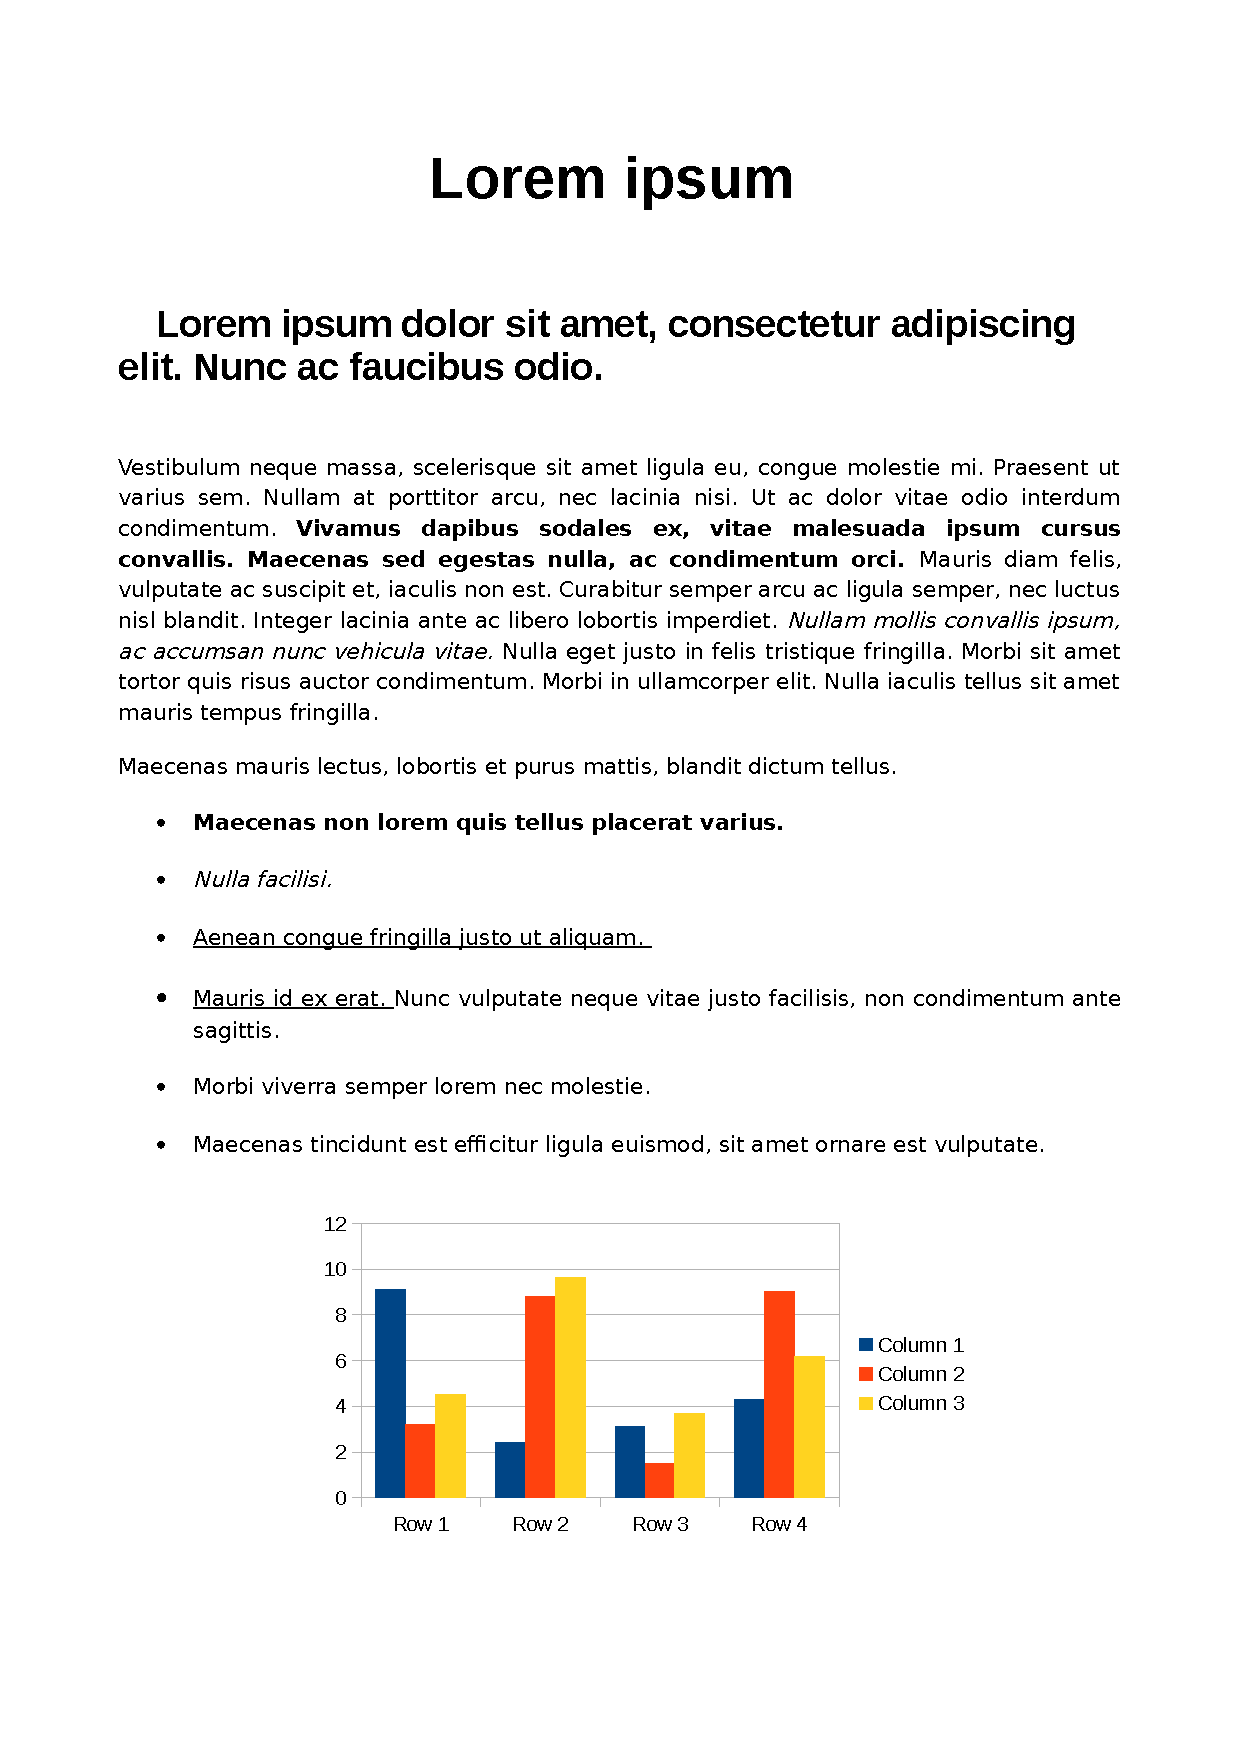
\includepdf[pages={1-}, scale=0.9]{res/documents/file-sample.pdf} % #appendix
%!TEX root = ../thesis.tex

%-----------------------------------------------------------------------------%
% MATHEMATICS
%-----------------------------------------------------------------------------%
%
% This module provides some packages for mathematical stuff like equations,
% matrices, etc.

\usepackage{amsmath}
\usepackage{amssymb} % #mathematics

%-----------------------------------------------------------------------------%
% FIXES
%-----------------------------------------------------------------------------%
% By default this template enables all fixes to improve the compiled result.
% However, if you have any problems or don't want the beheviour, just comment
% out the fix with a `%` sign.
% It is recommended to enable all fixes for the best results.
%!TEX root = ../../thesis.tex

%-----------------------------------------------------------------------------%
% This fix improves the typography and layout of the pdf file.
%-----------------------------------------------------------------------------%

% Fix: Pin chapter headings at top of page.
%\renewcommand*\chapterheadstartvskip{}

% Avoid `Schusterjungen` and `Hurenkinder`
\clubpenalty=10000
\widowpenalty=10000
%!TEX root = ../../thesis.tex

%-----------------------------------------------------------------------------%
% This fix adds support to sans serif fonts.
%-----------------------------------------------------------------------------%

% Load fonts
\usepackage{sourcesanspro}
\usepackage{sourcecodepro}

% Apply sans serif font as default
\renewcommand*{\familydefault}{\sfdefault}

% Set URL to sans serif font
\urlstyle{sf}
%!TEX root = ../../thesis.tex

%-----------------------------------------------------------------------------%
% This fix add a package `scrhack` to supress the deprecation warnings from
% inside the KOMA-scripts.
%-----------------------------------------------------------------------------%

\usepackage{scrhack}
%!TEX root = ../../thesis.tex

%-----------------------------------------------------------------------------%
% This fix uses the microtype package to enable better typography and decrease
% `Overfull` and `Underfull` information output from latex.
%
% If using a bibliography with the biblatex package, the url handling of xurl
% is borken. To solve this issue, load the xurl package after the biblatex
% package.
% https://tex.stackexchange.com/questions/3033/forcing-linebreaks-in-url
%-----------------------------------------------------------------------------%

% Enable better typograhpie to decrease `Overfull` and `Underfull` informations.
\usepackage[activate]{microtype}

% Load this package after `biblatex` to solve url linebreaking in the
% bibliography.
\usepackage{xurl}
%!TEX root = ../../thesis.tex

%-----------------------------------------------------------------------------%
% This fix provides internationalization for listings.
%-----------------------------------------------------------------------------%

\renewcommand{\lstlistingname}{\sListingPhrase}
\renewcommand{\lstlistlistingname}{\sListListingPhrase}

% Do not comment out this fixes, otherwise some other pieces would not work.
%!TEX root = ../../thesis.tex

%-----------------------------------------------------------------------------%
% Support multiple authors for thesis.
% Separate authors by a colon.
%-----------------------------------------------------------------------------%

% Check if multiple authors are included.
\newboolean{multipleAuthors}%
\IfCharInString{,}{\documentAuthor}{%
    \setboolean{multipleAuthors}{true}%
}{%
    \setboolean{multipleAuthors}{false}%
}%
%!TEX root = ../../thesis.tex

%-----------------------------------------------------------------------------%
% Add a new command \source to add sources to figures.
%-----------------------------------------------------------------------------%

% Add source to figures.
\newcommand{\source}[1]{%
    \footnotesize{\sSourcePhrase{}: #1}%
}%

%-----------------------------------------------------------------------------%
% BIBLIOGRAPHY
%-----------------------------------------------------------------------------%
% Add your bibliography files here...
%%%%%%%%%%%%%%%%%%%%%%%%%%%%%%%%%%%%%%%%%%%%%%%%%%%%%%%%%%%%%%%%%%%%%%%%%%%%%%%
% \addbibresource{docs/bibliography.bib} % #bibliography
%%%%%%%%%%%%%%%%%%%%%%%%%%%%%%%%%%%%%%%%%%%%%%%%%%%%%%%%%%%%%%%%%%%%%%%%%%%%%%%

%-----------------------------------------------------------------------------%
% GLOSSARIES
%-----------------------------------------------------------------------------%
% Add your glossaries and acronyms here...
%%%%%%%%%%%%%%%%%%%%%%%%%%%%%%%%%%%%%%%%%%%%%%%%%%%%%%%%%%%%%%%%%%%%%%%%%%%%%%%
% %!TEX root = ../thesis.tex

%-----------------------------------------------------------------------------%
% Defining new glossary entries
% \newglossaryentry{IDENTIFIER}{name=NAME, description=DESCRIPTION}
\newglossaryentry{mit-lizenz}{
    name=MIT-Lizenz,
    description={
        Die MIT-Lizenz ist eine permissive Open-Source-Lizenz, die es erlaubt,
        dieses Projekt zu verteilen, zu verändern und vieles mehr. Die volle
        Lizenz ist im Root-Verzeichnis dieses Projekts zu finden.
    }
}

\newglossaryentry{github}{
    name=GitHub,
    description={
        GitHub ist eine Plattform zur Versionsverwaltung von Softwareprojekten.
        Projekte sind dort in sogenannten \emph{Repositories} organisiert. Der
        Quellcode ist öffentlich. Eine entsprechende Lizenzierung ermöglicht
        die Nutzung dieser Softwareporjekte auch für eigene Projekte.
    }
}
%-----------------------------------------------------------------------------% % #glossaries
%%%%%%%%%%%%%%%%%%%%%%%%%%%%%%%%%%%%%%%%%%%%%%%%%%%%%%%%%%%%%%%%%%%%%%%%%%%%%%%

%-----------------------------------------------------------------------------%
% DOCUMENT
%-----------------------------------------------------------------------------%
\begin{document}
    % Site counter (recommended)
    \newcounter{savepage}

    % Cover
    %!TEX root = ../thesis.tex

%-----------------------------------------------------------------------------%
% COVER
%-----------------------------------------------------------------------------%
% This is a template for your titlepage.
% It is recommended to not change anything. In some cases the attribute of the
% company-logo must be adjusted. See the block below.
% In the `settings/metadata.tex` file you can manage which information are
% shown.
\begin{titlepage}

    % Show logos at the top of the document.
    \begin{center}
        \begin{minipage}{0.9\textwidth}
            \centering
            
            % Company logo
            \IfStrEq{\companyLogo}{yes}{%
                \raisebox{-0.5\height}%
                    %%%%%%%%%%%%%%%%%%%%%%%%%%%%%%%%%%%%%%%%%%%%%%%%%%%%%%%%%%%
                    % Change the `width` attribute to adjust it to your 
                    % purposes. You can also use the `hight` attribute instead.
                    %                [width=<value>
                    %                [height=<value>
                    %%%%%%%%%%%%%%%%%%%%%%%%%%%%%%%%%%%%%%%%%%%%%%%%%%%%%%%%%%%
                    {\includegraphics[width=0.2\textwidth]%
                    {res/logos/company.png}}
                \hfill
            }{}%
            % DHBW logo
            \IfStrEq{\dhbwLogo}{yes}{%
                \raisebox{-0.5\height}{%
                    %%%%%%%%%%%%%%%%%%%%%%%%%%%%%%%%%%%%%%%%%%%%%%%%%%%%%%%%%%%
                    % Change the `width` attribute to adjust it to your 
                    % purposes. You can also use the `hight` attribute instead.
                    %                [width=<value>
                    %                [height=<value>
                    %%%%%%%%%%%%%%%%%%%%%%%%%%%%%%%%%%%%%%%%%%%%%%%%%%%%%%%%%%%
                    \includegraphics[width=0.3\textwidth]%
                    {res/logos/dhbw.png}}
            }{}%
        \end{minipage}
    \end{center}

    % Some space between the header and the content.
    \vspace{5mm}

    % Title and general information
    \begin{center}
        \doublespacing{%
            \vspace*{5mm}{\LARGE\textbf{\documentTitle}}
        }%

        \vspace*{8mm}{\large\textbf{\sDocumentTypePhrase}}\\

        % Show degree if document is a bachelor thesis.
        \IfDocType{bachelor}{%
            \vspace*{6mm}{\sDegreePhrase}\\
            \vspace*{0mm}{\textbf{\degree}}\\
        }

        % Show lecture phrase only if set and not a bachelor thesis.
        \IfStrIsEmpty{\lecture}{}{% else
            \IfDocType{bachelor}{}{% else
                \vspace*{6mm}{\sLecturePhrase}\\
                \vspace*{0mm}{\textbf{\lecture}}\\
            }%
        }%

        \vspace*{8mm}{\sDepartmentPhrase{} \department}\\
        \vspace*{0mm}{\sLocationUniversityPhrase{} \locationUniversity}\\
        \vspace*{10mm}{\sDocumentAuthorPhrase}\\
        \vspace*{0mm}{\large \textbf{\documentAuthor}}\\
        
        \vfill

        \vspace*{0mm}{\releaseDate}\\

        \vfill

        % Show restriction notice if set
        \IfStrEq{\restricted}{yes}{%
            \vspace*{12mm}{\large\textbf{\sRestrictionNoticePhrase}}\\
        }{}%
    \end{center}

    % % Fill empty space
    % \vfill

    % % Additional information about the author, company and DH.
    % \begin{center}
    %     \begin{tabular}{ll}
    %         \textbf{\sDocumentPeriodPhrase} & \documentPeriod\\
    %         \textbf{\sMatriculationNumberPhrase, \sCoursePhrase} & %
    %             \matriculationNumber, \course\\
    %         % Show company information only if set
    %         \IfStrIsEmpty{\sCompanyPhrase}{}{% else
    %             \IfStrIsEmpty{\companyLocation}{}{% else 
    %                 \textbf{\sCompanyPhrase} & \companyName, %
    %                     \companyLocation\\
    %             }%
    %         }%
    %         \textbf{\sTutorPhrase} & \tutor\\
    %         % Show evaluator if bachelor thesis is set.
    %         \IfDocType{bachelor}{%
    %             \textbf{\sEvaluatorPhrase} & \evaluator
    %         }{}%
    %     \end{tabular}
    % \end{center}

\end{titlepage}

    %-------------------------------------------------------------------------%
    % Set site style to roman numbering
    \pagenumbering{roman}
    %-------------------------------------------------------------------------%

    % Restriction
    % Automatically disabled, if you set `\restrictedDocument` to `no`
    \IfStrEq{\restricted}{yes}{%
        %!TEX root = ../thesis.tex

\thispagestyle{empty}
\chapter*{\sRestrictionNoticePhrase}

\edef\RestrictionFile{res/i18n/\languageLongId/restriction_notice}%
\input{\RestrictionFile}

%!TEX root = ../thesis.tex

\vspace{3em}

% Set release date
\releaseLocation, \releaseDate
\vspace{4em}

% Space for authors signature
\rule{6cm}{0.4pt}\\
\documentAuthor
        \newpage
    }{}%

    % Declaration of honor
    % %!TEX root = ../thesis.tex

\thispagestyle{empty}
\chapter*{\sDeclarationPhrase}

\edef\DeclarationFile{res/i18n/\languageLongId/declaration}%
\input{\DeclarationFile}

%!TEX root = ../thesis.tex

\vspace{3em}

% Set release date
\releaseLocation, \releaseDate
\vspace{4em}

% Space for authors signature
\rule{6cm}{0.4pt}\\
\documentAuthor
    % \newpage

    %%%%%%%%%%%%%%%%%%%%%%%%%%%%%%%%%%%%%%%%%%%%%%%%%%%%%%%%%%%%%%%%%%%%%%%%%%%
    % Abstract
    %%!TEX root = ../thesis.tex

%-----------------------------------------------------------------------------%
% Here you can define your abstract in various languages, following this
% examples.
% Make sure, that you included the `abstract` package in your document file.
%-----------------------------------------------------------------------------%

\begin{otherlanguage}{ngerman}
	\begin{abstract}
		Dieses Dokument bietet einen Überblick über verschiedene Funktionen der
        Vorlage für Projektarbeiten an der \acs{dhbw}. Gleichzeitig wurde
        dieses Dokument mithilfe der Vorlage für Projektarbeiten erstellt und
        dient damit als kleine Dokumentation und als Nachschlagewerk für
        verschiedene \LaTeX{}-Kommandos, um einen schnellen Einstieg auch ohne
        Vorkenntnisse in \LaTeX{} zu ermöglichen.
		
		Das Projekt selbst steht unter einer \Gls{mit-lizenz} und kann daher von
        jedem frei verwendet werden. Wenn du selbst Verbesserungsvorschläge
        hast oder dich an dem Projekt beteiligen willst, fühle dich frei, auf
        \Gls{github} ein \emph{Issue} oder direkt ein \emph{Pull Request} zu
        öffnen, sodass diese Vorlage weiterhin stetig verbessert wird. Zum 
        \Gls{github}-Repository gelangst du mit folgender \ac{url}: 
		\url{https://github.com/dateiexplorer/dhbw-latex-template}.
	\end{abstract}
\end{otherlanguage}

\begin{otherlanguage}{english}
	\begin{abstract}
		This document provides an overview of various functions of the template
        for thesises at the \acs{dhbw}. Furthermore, this document was
        created using the template for thesises and thus serves as a small
        documentation and as a reference for various \LaTeX{} commands to get a
        quick entry even without prior knowledge about \LaTeX{}.
		
		The project itself is licensed under MIT and can therefore be used
        freely by anyone. If you have any suggestions for improvement or if you
        want to contribute to the project feel free to open an \emph{Issue} or
        directly a \emph{Pull Request} on \Gls{github}, so that this template
        will continue to be constantly improved. You can get to the \Gls{github}
        repository with the following \ac{url}: 
		\url{https://github.com/dateiexplorer/dhbw-latex-template}.
	\end{abstract}
\end{otherlanguage}

%-----------------------------------------------------------------------------%
% Add more abstracts... % #abstract
    %%%%%%%%%%%%%%%%%%%%%%%%%%%%%%%%%%%%%%%%%%%%%%%%%%%%%%%%%%%%%%%%%%%%%%%%%%%

    % Don't show header in indices
    \pagestyle{empty}

    %-------------------------------------------------------------------------%
    % INDICES
    %-------------------------------------------------------------------------%
    % \tableofcontents
    
    % Acronyms
    % \addchap{\sAcronymPhrase} % #acronyms
    %%%%%%%%%%%%%%%%%%%%%%%%%%%%%%%%%%%%%%%%%%%%%%%%%%%%%%%%%%%%%%%%%%%%%%%%%%%
    % %!TEX root = ../thesis.tex

%-----------------------------------------------------------------------------%
% ACRONYMS
%-----------------------------------------------------------------------------%
% Make acronyms
\usepackage[printonlyused]{acronym}
 % #acronyms
    %%%%%%%%%%%%%%%%%%%%%%%%%%%%%%%%%%%%%%%%%%%%%%%%%%%%%%%%%%%%%%%%%%%%%%%%%%%

    % \listoffigures
    % \listoftables
    % \lstlistoflistings % #listings

    % Set site style to arabic numbering
    \cleardoublepage
    \setcounter{savepage}{\arabic{page}}
    \pagenumbering{arabic}

    % Enable header
    \pagestyle{fancy}
    \fancyhf{}
    \fancyhead[L]{\documentAuthor}
    \fancyhead[R]{\documentTitle}

    %-------------------------------------------------------------------------%
    % CONTENT
    %-------------------------------------------------------------------------%
    %!TEX root = ../thesis.tex

%-----------------------------------------------------------------------------%
% Add all your main content files here.
%
% It is recommended to use a separate `content/` folder and put all your tex
% files there.
%-----------------------------------------------------------------------------%

% Comment this files out for your thesis.
% %!TEX root = ../../thesis.tex

\chapter{Über dieses Projekt}
    
Ziel dieses Projekts ist es, eine leichtgewichtige und moderne 
\LaTeX{}-Vorlage für wissenschaftliche Arbeiten an der \ac{dhbw}
bereitzustellen. Dabei soll \LaTeX{} vor allem auch für Neulinge zugänglich 
gemacht werden, sodass die Hürde der Einarbeitung möglichst gering wird. 
Deshalb ist sämtlicher \LaTeX{}-Code ausführlich dokumentiert, sodass alle 
Funktionen genau erläutert werden.

Diese \LaTeX{}-Vorlage wird von Grund auf neu geschrieben und hat das Ziel, 
so wenige Pakte wie möglich einzubinden und diese so zu strukturieren, dass 
sie modular inkludiert werden können.

Dieses Dokument selbst dient nicht primär zur Dokumentation des Codes, 
sondern stellt lediglich einige Beispiele bereit, um alle benötigten 
Funktionen für das Schreiben einer wissenschaftlichen Arbeit vorzustellen.
Dabei wurde dieses Dokument selbst mit der Vorlage erstellt.
Dieses Dokument ist also viel mehr als eine Sammlung zu verstehen, in der
nachgeschlagen werden kann, wenn eine bestimmte Funktion in eigenen
Arbeiten übernommen werden soll. Jede Funktion hat hierfür ein eigenes 
Kapitel. Größere Themenkomplexe sind in Kapitel und Unterkapitel 
aufgeteilt. Dieses Dokument zeigt also, wie eine wissenschaftliche Arbeit
aussehen könnte.

\section{Disclaimer}

Vorweg: Diese Vorlage ist keine offizielle Vorlage irgendeiner \ac{dhbw}.
Deshalb erhebt sie auch keinen Anspruch auf Vollständigkeit oder
Richtigkeit. Es sollten vorher die Anforderungen an die Arbeit bei der
Hochschule geprüft werden. Ggf. müssen einige Änderungen vorgenommen werden.
Dennoch versucht diese Vorlage die Grundanforderungen der \ac{dhbw}
umzusetzen.

\section{Entwicklung}

Dieses Projekt steht unter der \Gls{mit-lizenz}. Damit steht dieses Projekt
jedem (zur Nutzung und zur Weiterentwicklung) frei zur Verfügung. Genauere
Details zur Lizenz finden sich in einer entsprechenden separaten Datei.

Natürlich steht es jedem frei, an dieser Vorlage selbst weiterzuentwickeln.
Dabei möchte ich jedoch darauf hinweisen, dass viele Probleme eventuell auch
andere Studenten betreffen. Deshalb ist es ausdrücklich erwünscht,
Weiterentwicklungen der Vorlage oder bestimmte Features per Pull Request
wieder in dieses Repository zurückfließen zu lassen. Diese Vorlage ist ein
Community-Projekt und lebt davon, dass es viele Entwickler gibt, die ihren
Teil dazu beitragen.
% %!TEX root = ../../thesis.tex

\chapter{Basics}

In diesem Kapitel werden nun die grundlegenden \LaTeX{}-Funktionen vorgestellt.
Es wird empfohlen, einzelne Textbausteine in den Quelldateien nachzulesen, da
dort einige weitere Informationen zu finden sind.

\section{Kompilieren einer \LaTeX{}-Datei}

Zunächst ist wichtig zu verstehen, dass es sich bei den \emph{.tex} Dateien um
ganz normale Textdateien handelt, die mit einem herkömlichen Texteditor
einsehen und bearbeiten lassen. Damit ist \LaTeX{} unabhängig von irgendeiner
zusätzlichen Software. Dateien können auch komplett im Terminal mit Texteditoren
wie \emph{nano} oder \emph{vim} unter Linux entwickelt werden.
Diese Textdateien werden anschließend mit einem Programm kompiliert, um daraus
eine PDF-Datei zu erzeugen.

\section{Texte schreiben}

In einer TEX-Datei kann schließlich ganz normaler Text geschrieben werden. Dabei
werden Zeichenumbrüche ignoriert. Das schöne ist, dass \LaTeX{} sich um das
Layout und das Setzen des Textes kümmert. Das heißt, es ist egal, wie unsere
Quelldatei letztlich formatiert ist, am Ende erhält man immer ein Ergebnis, das
nach typographischen Regeln gut aussehen wird.

Mit verschiedenen Commands können Texte auch angepasst werden, dabei wird
mit den Commands immer eine semantische Bedeutung gegeben. Das Command
\code{\textbackslash{}emph} weist \LaTeX{} beispielsweise dazu an, einen Text
hervorzuheben. Standardmäßig wird das durch das kursive Setzen des
entsprechenden Textes bewerkstelligt.

Mit einer leeren Zeile wird \LaTeX{} mitgeteile, dass nun ein neuer Absatz
erfolgen soll. In dieser Vorlage ist standardmäßig eingestellt, dass ein neuer
Absatz durch einen kleinen Zwischenraum abgetrennt wird. In der
Standardeinstellung eines normalen \LaTeX{}-Dokuments, das nicht mit dieser
Vorlage erstellt wird, wird der Absatz eingerückt (wie man es von Büchern her
kennt). In wissenschaftlichen Arbeiten ist dieses Verhalten aber eher unüblich.
Letztlich ist es aber Geschmackssache und jeder kann die Vorlage nach seinen
Wünschen anpassen.

\section{Aufzählungen}

In \LaTeX{} können auch verschiedene Auflistungen gemacht werden. Diese
Aufzählungen können nummeriert oder unnummeriert sein.

Ungeordnete Liste:
\begin{itemize}
    \item Item 1
    \item Item 2
    \item Item 3
\end{itemize}

Geordnete Liste:
\begin{enumerate}
    \item Item 1
    \begin{enumerate}
        \item Item 1.1
        \item Item 1.2
        \item Item 1.3
    \end{enumerate}
    \item Item 2
    \item Item 3
\end{enumerate}

Außerdem gibt es die Möglichkeit, eine Aufzählung von Worten und einer
Beschreibung zu generieren.

\begin{description}
    \item[Item 1] \hfill \\
        Beschreibung des ersten Items in der Liste. Diese Beschreibung kann auch
        über mehrere Zeilen gehen.
    \item[Item 2] \hfill \\
        Beschreibung des zweiten Items...
    \item[Item 3] \hfill \\
        Beschreibung des dritten Items...
\end{description}
% %!TEX root = ../../thesis.tex

\chapter{Bilder einfügen}

Im Folgenden wird ein ein Bild eingefügt. Diese Bild zeigt das Maskottchen
von Linux, einem Pinguin. Der Pinguin sollte glücklich aussehen, so als
hätte er gerade eine Maß Bier genossen und den besten Sex seines Lebens
gehabt \parencite[]{tux2021}.

\begin{figure}[ht]
    \centering
    
\includegraphics[width=5cm]{res/images/tux.png}
    \caption{Tux - Das Maskottchen von Linux}
\end{figure}
% %!TEX root = ../thesis.tex

%-----------------------------------------------------------------------------%
% LISTINGS
%-----------------------------------------------------------------------------%
\usepackage{listings}

\lstdefinestyle{defaultstyle}{
    backgroundcolor=\color{background},
    numberstyle=\tiny\color{codegray},
    basicstyle=\footnotesize\ttfamily,
    breakatwhitespace=false,
    breaklines=true,
    captionpos=t,
    keepspaces=true,
    numbers=left,
    numbersep=5pt,
    showspaces=false,
    showstringspaces=false,
    showtabs=false,
    tabsize=4
}

\lstset{style=defaultstyle}

% Sample files for a technical project thesis.
% \input{content/main/introduction}
% \input{content/main/technologies}
% \input{content/main/evaluation}
% \input{content/main/conceptual_design}
% \input{content/main/implementation}
% \input{content/main/conclusion}

%!TEX root = ../thesis.tex

\section{Metapher}

Der Ant-Colony-Optimization-Algorithmus (ACO) ist von dem sozialen Verhalten
von Insekten und insbesondere von Ameisen inspiriert. Dabei ist ein
Individuum einer Kolonie wenig komplex, durch das Zusammenspiel aller
Individuen sind Ameisen allerdings in der Lage, gemeinsam komplexe Aufgaben
zu bewältigen.

Der hier vorgestellte Algorithmus lässt sich von der Futtersuche von Ameisen
ableiten. Das Verhalten wird in dem sog. \emph{Double-Bridge-Experiment}
analysiert. Dabei haben Ameisen genau zwei Wege, um von ihrem Nest zu einer
Futterquelle zu gelangen. Einer der beiden Wege ist dabei länger als der
andere. Zu Beginn schwärmen die Ameisen aus und nutzen beide Wege, um zu
der Futterquelle zu gelangen. Nach einiger Zeit wird man allerdings
beobachten, dass sich eine Ameisenstraße über den kürzeren der beiden Wege
bildet. Die Ameisen nutzen also eine Strategie, um den schnellsten Weg von
ihrem Nest zum Futter zu finden.
Diese Strategie ist maßgeblich auf das Schwarmverhalten und ausgesetzte
Pheromonspuren zurückzuführen. Finden Ameisen Futter, so kommunizieren sie
den Weg ihren Artgenossen durch einen Duftstoff über den Weg, den sie
gelaufen sind. Andere Ameisen folgend schließlich dieser Duftspur und
gelangen ebenfalls an das Futter. Kürzer Wege werden so öfter frequentiert
von Ameisen abgelaufen, wodurch die Pheromonspur auf diesem Weg stärker wird.
Die Pheromonspur verfliegt mit der Zeit auf den anderen Wegen.
So nehmen immer mehr Ameisen die kürzeste Strecke und es bilden sich 
die typischen Ameisenstraßen.
Damit nutzen Ameisen ihr Schwarmverhalten, um den Weg von ihrem Nest zur
Futterstelle zu optimieren. Eine Eigenschaft, die sich auch für das TSP
zunutze gemacht werden kann.

\section{Strategie}

Die Strategie für diesen Algorithmus liegt darin, dass sowohl das kollektive
Schwarmverhalten durch die Pheromonspur genutzt wird (historischen Information),
um bekannte Wege zu exploitieren und den günstigsten Pfad zu finden, als auch
ein individuelles Verhalten in die Wegfindung einzelner Ameisen mit einfließt,
das durch eine einfache Heuristik simuliert wird (heuristische Informationen).

Ameisen laufen zunächst zufällig verschiedene Pfade iterativ ab und 
teilen die Pheromoninformationen über das kollektive Gedächtnis mithilfe einer 
Pheromonmatrix, die jeder Ameise zur Verfügung steht. Auf diese Weise lässt 
sich effektiv ein Optimum für den gewünschten Suchraum finden.

\section{Prozedur}
\label{sec:prozedur}

Für das kollektive Gedächtnis wird eine Pheromonenmatrix angelegt, die die
Pheromonenwerte aller Kanten eines Graphen beinhalten. Diese Werte fließen
in die Entscheidung für einen Knotenpunkt bei jeder Iteration mit ein. Die
Pheromonenmatrix ist dabei das kollektive Gedächtnis der Ameisenkolonie.
Jede Ameise nutzt außerdem eine Metaheuristik, mit der sie selbstständig einen
nächsten Knotenpunkt auswählt. Beide Faktoren können gewichtet werden, um
ihren jeweiligen Einfluss auf die Entscheidung einer einzelnen Ameise zu
steuern.
Daraus lässt sich ein stochastisches Modell entwickeln, das sich mathematisch
folgendermaßen ausdrücken lässt:
\begin{equation}
    p_{i,j}^k(t) = \frac{\tau_{i,j}^\alpha * \eta_{i,j}^\beta}{
        \sum_{k=1}^c \tau_{i,k}^\alpha * \eta_{i,k}^\beta
    }
\end{equation}

Dabei ist $p_{i,j}$ die Wahrscheinlichkeit, mit der die Kante des Graphen
von Position $i$ nach Position $j$ von einer Ameise gelaufen wird,
$\tau_{i,j}$ ist die Pheromoninformation für diese Kante und wird über das
kollektive Gedächtnis mit allen Ameisen geteilt, $\eta_{i,j}$ ist die
heuristische Information, die beispielsweise durch die Berechnung der
Euklidischen Distanz zwischen den einzelnen Punkten $i$ und 
$j$ im Graph berechnet wird;
$\alpha$ ist die Gewichtung, mit der die Pheromoninformationen, also das
kollektive Gedächtnis, auf die Entscheidung der Ameise Einfluss nehmen und
$\beta$ ist entsprechend die Gewichtung für die Einflussnahme der Heuristik,
also dem individuelle Verhalten, auf die Entscheidung.
Um bessere Ergebnisse zu erzielen, werden die Ergebnisse außerdem ins
Verhältnis zu den Ergebnissen aller Ameisen gesetzt.
Dabei ist $k$ der Index einer virtuellen Ameise, $c$ die 
gesamte Anzahl der Ameisen, $\tau_{i,k}$ die Pheromonenmatrix
und $\eta_{i,k}$ die gesamten Distanzen.

Mit dieser grundlegenden Formel lassen sich verschiedene Pfade im
gewünschten Suchraum ablaufen.
Nach jeder Iteration werden die Pheromonenwerte in der Pheromonenmatrix
aktualisiert. Wird die maximale Anzahl an Iterationen erreicht oder das
Optimum ändert sich nicht oder nur geringfügig, ist das Optimum gefunden.
Der Algorithmus liefert den Pfad, der nach der letzten Iteration als
bester Pfad ausgewählt wurde. Das ist derjenige, auf dem die höchste
Pheromonkonzentration zu finden ist.

\section{Pseudocode}

Der Hauptteil des ACO ist eine einfache \code{while}-Schleife, die solange
durchlaufen wird, bist eine Abbruchbedingung erfüllt ist. Diese kann
beispielsweise durch eine maximale Anzahl an Iterationen festgelegt werden
oder durch einen Fitness-Wert, der die Veränderung zum vorherigen Ergebnis
angibt. Fällt dieser Werte unter eine bestimmte Schranke, ist das Ergebnis
nah genug am Optimum und der Algorithmus kann terminiert werden.
Für den Algorithmus ergibt sich folgender Pseudocode:

\begin{lstlisting}
    while (Abbruchbedingung trifft nicht zu) do
        GenerierePfadeFuerAmeisen();
        AktualisierePheromone();
        AktualisiereMomentanesOptimum();
    done
\end{lstlisting}

In jedem Durchlauf läuft jede Ameise mithilfe der in Abschnitt
\ref{sec:prozedur} beschriebenen Formel einen gesamten Pfad für das TSP ab
(\emph{GenerierePfadeFuerAmeisen}).
Anschließend wird die Pheromonmatrix für den nächsten Durchlauf aktualisiert.
In diesem Schritt wird auch ein \emph{evaporation}-Faktor (Verdampfung)
angewendet, der angibt, wie viel vom ursprünglichen Pheromonenwert pro
Kante für die nächste Iteration behalten wird (\emph{AktualisierePheromone}).
Damit werden weniger
frequentierte Kanten schneller im kollektiven Gedächtnis als
nichtzielführend markiert, wodurch der Algorithmus schneller ein globales
Optimum finden kann.
Außerdem lässt sich der Algorithmus dadurch nicht nur für statische Probleme,
wie dem TSP, sondern auch für dynamische Probleme einsetzen, beispielsweise
die Routenfindung in Navigationssystemen mit sich ändernden Positionsdaten.
Würden sich Ausgangsparameter ändern, kann über die \emph{evaporation}
sichergestellt werden, dass ursprüngliche vielversprechende Lösungen, die
durch die Parameteränderung nicht mehr zielführend sind, mit der Zeit wieder
vergessen werden.
Am Ende jedes Durchlaufs wird der beste Pfad aller bisher von den Ameisen
durchlaufenden Pfaden ermittelt (\emph{AktualisiereMomentanesOptimum}).
Dieser stellt das momentane gefundene globale Optimum dar.

\section{Exploration and Exploitation}

Die Exploration, also das zufällige Erkunden des neuen 
Suchraums, wird maßgeblich durch die Gewichtung $\beta$ der Metaheuristik 
beeinflusst (heuristische Komponente). Die Erkundung geschieht dadurch,
dass Ameisen an jedem Knotenpunkt im Graphen wahrscheinlichkeitsbasiert
auswählen, welche Kante sie entlanggehen. 
Je höher $\beta$ im Gegensatz zu $\alpha$ gewählt wird, desto mehr Suchraum wird 
exploriert, allerdings leidet darunter die Exploitation.
Diese wiederum wird durch die Gewichtung $\alpha$ beeinflusst. Mithilfe
von $\alpha$ wird der Einfluss des kollektiven Gedächtnisses in die Wegfindung
der Ameise gesteuert (historische Komponente).
Ein ausgeglichenes Verhältnis zwischen $\alpha$ und $\beta$ ist zu wählen, um
die Suche nach einem Optimum möglichst effizient zu gestalten.

\section{Entscheidungsregeln für Schwarmverhalten}

Ameisen im ACO nutzen zum einen das kollektive Gedächtnis, um
wahrscheinlichkeitsbasiert an jedem Knotenpunkt eines Graphen die nächste
Kante auszuwählen ($\tau$), zum anderen eine Metaheuristik ($\eta$), um ein
individuelles Verhalten einer Ameise zu simulieren.
Welche Kante eine Ameise bei der Wegfindung als nächstes auswählt, wird
durch die Wahrscheinlichkeit $p_{i,j}$ festgelegt, deren Berechnung bereits
in Abschnitt \ref{sec:prozedur} erläutert wurde.
Wie stark die historischen und heuristischen Komponenten einen Einfluss auf
die Wegfindung einer Ameise haben, hängt von
den Gewichtungsfaktoren $\alpha$ und $\beta$ ab. Wird $\alpha$ beispielsweise
auf 0 gesetzt, so fließen die Informationen des kollektiven Gedächtnisses und
damit die Pheromoninformationen nicht in die Wegfindung mit ein. Eine Ameise
wird also einen Weg wählen, der nur auf der aktuellen Distanz zu einem nächsten
Knotenpunkt basiert. Damit gleicht das Suchen eines Optimums einer Suche mit
Bruteforce und ist nicht effizient. Wird hingegen $\beta$ auf 0 gesetzt, so
berücksichtigt eine Ameise nur die Pheromoninformationen, wodurch keine neuen
Wege mehr exploriert werden. Es besteht die Gefahr, dass das globale Optimum
nicht gefunden wird, da jegliches individuelle Verhalten fehlt.
Deshalb ist bei der Wahl von $\alpha$ und $\beta$ ist ein ausgewogendes
Verhältnis zwischen diesen Parametern notwendig, um eine möglichst effiziente
Suche zu gewährleisten.

\section{Parameterabhängigkeiten}

Für den ACO können diverse Startparameter definiert werden. 
So legt $\alpha$ die Gewichtung für die Exploitation~--~also den Einfluss der
Pheromoninformation bei der Wegfindung~--~und $\beta$ die Gewichtung der
Exploration~--~also das zufällige Wählen eines Pfades basierend auf der
Metaheuristik~--~fest. Außerdem kann mithilfe des Parameters
\emph{evaporation} ($\rho$) angegeben werden, wie viel Prozent
des ursprünglichen Pheromonwerts nach einer Iteration behalten werden. Damit
wird das Verfliegen des Duftstoffes simuliert. Ein höherer Wert lässt die
Pheromonenwerte kleiner werden, dadurch kann angepasst werden, wie stark
auch niedrigfrequentierte Pfade in der nächsten Iteration zur Suche nach einem
Optimum miteinbezogen werden. Es sollten eher geringe Werte gewählt werden.
Bei einer \emph{evaporation} von 1.0 (100\%) werden nach jeder Iteration die
Pheromone zurückgesetzt, wodurch das kollektive Gedächtnis nach jeder Iteration
gelöscht wird. Das hat zur Folge, dass der Algorithmus nicht das globale
Optimum finden kann und Ameisen eine Bruteforce-Suche im gesamten Suchraum
starten.

Mit einem weiteren Parameter $q$ kann definiert werden, wie viele
Pheromone von einer einzelnen Ameise auf einem Pfad liegengelassen wird. Ein
höherer Wert führt zu einer höheren \glqq Auflösung\grqq in der Pheromonmatrix.
Wird beispielsweise $q=1$ gewählt und es laufen 10 Ameisen eine Kante entlang,
beträgt der Pheromonwert dieser Kante nach der ersten Iteration zunächst 10.
Durch die \emph{evaporation}, die in diesem Beispiel auf 0.1 (10\%) gesetzt
werden soll, wird der Pheromonwert dieser Kante schließlich den Wert 9
annehmen. Die Differenz zwischen diesen beiden Werten ist 1.
Wird hingegen $q=10$ gewählt, so nimmt der Pheromonwert dieser Kante den
Wert 100, bzw. nach der Verdampfung 90 an. Die Differenz der beiden Werte
(vor und nach der Verdampfung) beträgt hier bereits 10.
Das hat zur Folge, dass höhere Werte für $q$ eine größere Unterscheidung von
Pheromonwerten in der Matrix hat, wodurch die Intensität, die ein potentiell
guter Pfad für das Optimum auf das kollektive Gedächtnis hat, verstärkt wird.

Mit dem \emph{antFactor} lässt sich berechnen, wie viele Ameisen in Abhänigkeit
von Knotenpunkten für den Algorithmus erzeugt werden. Hier sollte ein Wert
zwischen 0.6 und 0.8 gewählt werden. Ein Wert von 0.6 würde bedeuten, dass für
60\% von Knotenpunkten, Ameisen erstellt werden, bei einer Anzahl von 100
Knoten in einem Graphen also 60 Ameisen zur Verfügung stehen, um das Optimum
für diesen Graphen zu finden. Mit diesem Parameter kann die Effizient des
Algorithmus gesteigert werden, da nicht für jeden Knotenpunkt eine Ameise zur
Verfügung stehen muss, wodurch die Komplexität reduziert und die
Geschwindigkeit bei der Ausfürhung des ACO erhöht wird.

Der \emph{randomFactor} kann verwendet werden, um bei der Auswahl von
nächsten Knotenpunkten einen kleinen Zufall einzubauen, wodurch die Exploration
erhöht wird, da Ameisen nicht unbedingt der nach der in Abschnitt
\ref{sec:prozedur} vorgestellten Wahrscheinlichkeitsberechnung besten Weg
nehmen müssen.

Zuletzt kann mit dem Parameter \emph{maximumIterations} festegelgt werden,
wie viele Iterationen durchlaufen werden sollen, bevor der Algorithmus
terminiert wird. Dies verhindert, dass ein Algorithmus nicht terminiert, wenn
keine Lösung gefunden wird, bzw. die gefundene Lösung noch nicht dem globalen
Optimum entspricht, eine weitere Suche das Ergebnis aber nicht erheblich
verbessern würde.

\section{Zusammenspiel \emph{Ant} und \emph{AntColony}}

Bei einer Konfiguration von $\alpha = 2$ und $\beta = 2$, werden $\tau$ und
$\eta$ gleichermaßen berücksichtigt. Damit wird sowohl das kollektive,
historische Gedächtnis der gesamten Kolonie (Pheromonenmatrix), als auch
das individuelle Verhalten einer einzelnen Ameise (Metaheuristik) in die
Wegfindung mit einbezogen. Dies führt zu einer
ausgewogenen Exploration und Exploitation des Suchraums, bei der einzelne
Individuen kollektiv zusammenarbeiten. Mit einer
Konfiguration, in der die \emph{evaporation} auf 0.05 gesetzt wird, werden
die Werte in der Pheromonenmatrix nach jeder Iteration um 5\% gesenkt. Es
werden also nur 95\% der eigentlichen Pheromonenwerte für die nächste
Iteration übernommen. Das hat zur Folge, dass Wege, die einmal von der
Kolonie als vielversprechend angesehen wurden, mit der Zeit auch wieder
vergessen werden können, wenn ein anderer, besserer Weg gefunden wird. Das
erhöht die Leistungsfähigkeit des ACO. Mit dem Wert \emph{q} = 500 wird für
jede Ameise,
die eine Kante des Graphen entlanggeht, der Pheromonwert für diese Kante um
500 erhöht. Damit lässt sich eine gute Auflösung der Pheromonenmatrix
erzielen. Der \emph{antFactor} von 0.8 sorgt dafür, dass für 80\% des
Suchraums, Ameisen erzeugt werden, die den gesamten Suchraum erkunden. Im
Falle des TSP würden bei 100 Städten also die Ameisenkolonie eine Größe von
80 Ameisen annehmen, wobei
jede Ameise in jeder Iteration einen Pfad für das TSP sucht und die neu
gewonnenen Informationen dem kollektiven Gedächtnis der Kolonie beisteuert.
Ein höherer Wert erhöht die Komplexität pro Iteration, ein niedrigerer Wert
erhöht hingegen die Anzahl an Iterationen, dafür wird die Rechenaufwand pro
Iteration minimiert.
Ein \emph{randomFactor} von 0.01 fügt der Auswahl bei der Wegfindung von
Ameisen für den nächsten Knotenpunkt eine Variation hinzu. Mit einer
Wahrscheinlichkeit von 1\% wählt die Ameise also einen anderen Knoten, als
den, den sie aufgrund der Berechnung gewählt hätte.


    % Change site style to roman numbering
    \cleardoublepage
    \pagenumbering{roman}
    \setcounter{page}{\thesavepage}

    %-------------------------------------------------------------------------%
    % BIBLIOGRAPHY
    %-------------------------------------------------------------------------%
    % \printbibliography % #bibliography

    %-------------------------------------------------------------------------%
    % GLOSSARY
    %-------------------------------------------------------------------------%
    % \printglossary % #glossaries

    %-------------------------------------------------------------------------%
    % APPENDIX
    %-------------------------------------------------------------------------%
    %%%%%%%%%%%%%%%%%%%%%%%%%%%%%%%%%%%%%%%%%%%%%%%%%%%%%%%%%%%%%%%%%%%%%%%%%%%
    % Change the appendix file here.
    \newcommand{\setAppendixFile}{content/appendix} % #appendix
    %%%%%%%%%%%%%%%%%%%%%%%%%%%%%%%%%%%%%%%%%%%%%%%%%%%%%%%%%%%%%%%%%%%%%%%%%%%
    \IfFileExists{\setAppendixFile}{%
        \appendixwithtoc

        \input{\setAppendixFile} % #appendix
    }{}
    
    % Site for cd if electronic version is enabled.
    \IfStrEq{\electronicVersion}{yes}{%
        %!TEX root = ../thesis.tex

\thispagestyle{empty}
\chapter*{\sDataCarrierPhrase}

%
    }{}%
\end{document}
